\documentclass{standalone}
\usepackage{tikz}
\usetikzlibrary{patterns, positioning}

\begin{document}
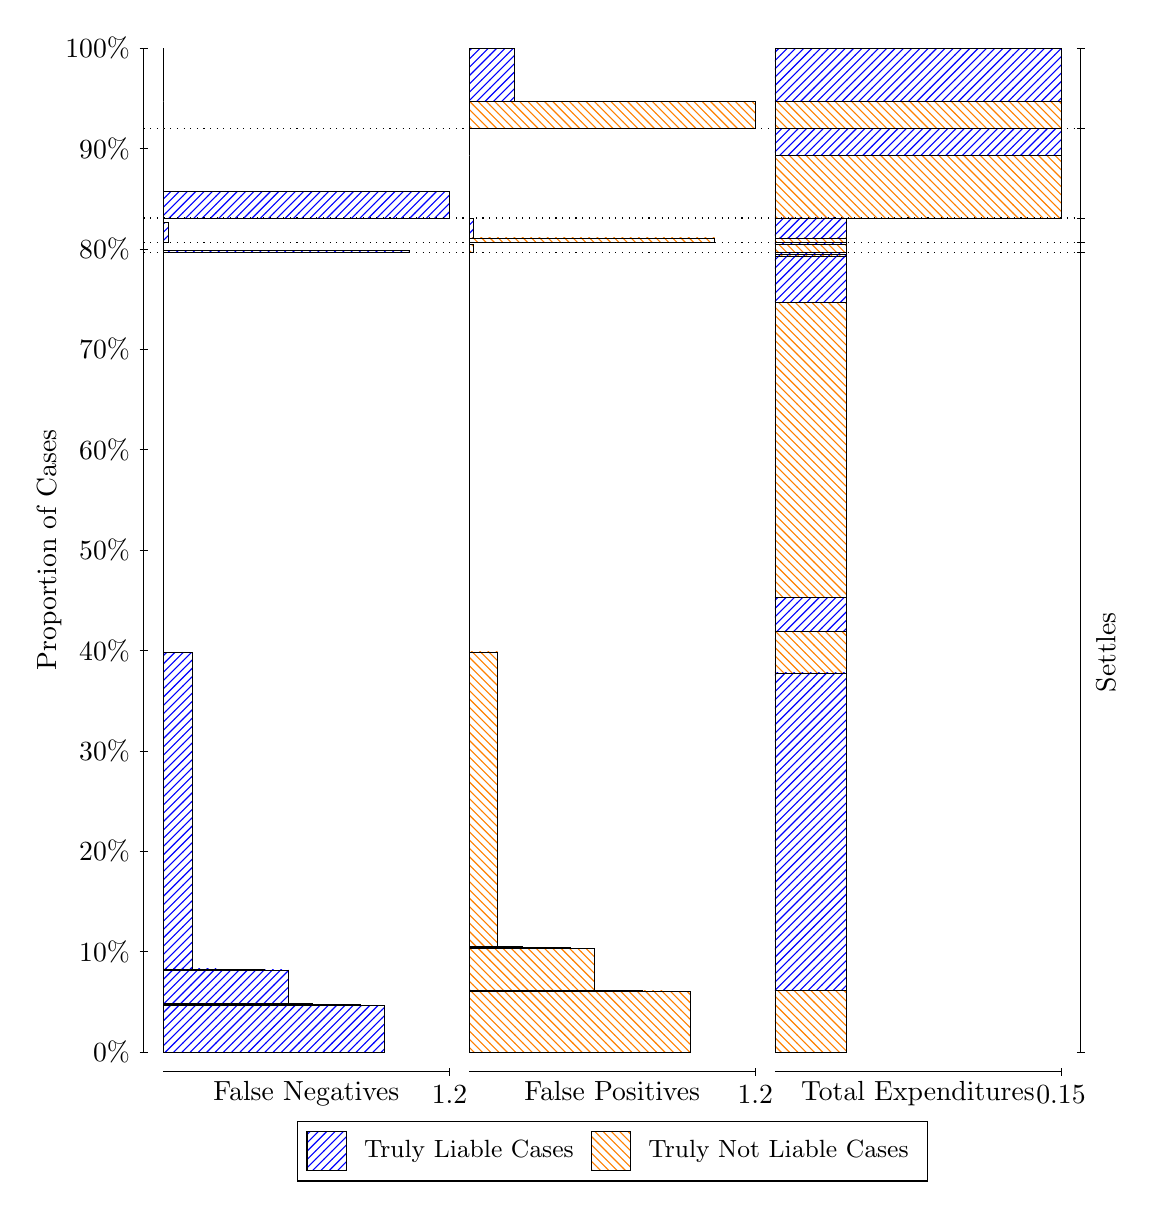
\begin{tikzpicture}
\draw[black, very thin] (1.5,1.75) -- (1.5,14.5);
\node[rotate=90, anchor=center] at (0.3, 8.125) {Proportion of Cases};
\draw[black, very thin] (1.45,1.75) -- (1.55,1.75);
\node[anchor=east] at (1.45, 1.75) {0\%};
\draw[black, very thin] (1.45,3.025) -- (1.55,3.025);
\node[anchor=east] at (1.45, 3.025) {10\%};
\draw[black, very thin] (1.45,4.3) -- (1.55,4.3);
\node[anchor=east] at (1.45, 4.3) {20\%};
\draw[black, very thin] (1.45,5.575) -- (1.55,5.575);
\node[anchor=east] at (1.45, 5.575) {30\%};
\draw[black, very thin] (1.45,6.85) -- (1.55,6.85);
\node[anchor=east] at (1.45, 6.85) {40\%};
\draw[black, very thin] (1.45,8.125) -- (1.55,8.125);
\node[anchor=east] at (1.45, 8.125) {50\%};
\draw[black, very thin] (1.45,9.4) -- (1.55,9.4);
\node[anchor=east] at (1.45, 9.4) {60\%};
\draw[black, very thin] (1.45,10.675) -- (1.55,10.675);
\node[anchor=east] at (1.45, 10.675) {70\%};
\draw[black, very thin] (1.45,11.95) -- (1.55,11.95);
\node[anchor=east] at (1.45, 11.95) {80\%};
\draw[black, very thin] (1.45,13.225) -- (1.55,13.225);
\node[anchor=east] at (1.45, 13.225) {90\%};
\draw[black, very thin] (1.45,14.5) -- (1.55,14.5);
\node[anchor=east] at (1.45, 14.5) {100\%};

\draw[black, very thin] (13.4,1.75) -- (13.4,14.5);
\draw[black, very thin] (13.35,1.75) -- (13.45,1.75);
\node[anchor=west] at (13.35, 1.75) {};
\draw[black, very thin] (13.35,11.904) -- (13.45,11.904);
\node[anchor=west] at (13.35, 11.904) {};
\draw[black, very thin] (13.35,12.034) -- (13.45,12.034);
\node[anchor=west] at (13.35, 12.034) {};
\draw[black, very thin] (13.35,12.342) -- (13.45,12.342);
\node[anchor=west] at (13.35, 12.342) {};
\draw[black, very thin] (13.35,13.478) -- (13.45,13.478);
\node[anchor=west] at (13.35, 13.478) {};
\draw[black, very thin] (13.35,14.5) -- (13.45,14.5);
\node[anchor=west] at (13.35, 14.5) {};

\draw[black, very thin, pattern color=blue, pattern=north east lines] (1.75,1.75) rectangle (4.5611,2.3442);
\draw[black, very thin, pattern color=blue, pattern=north east lines] (1.75,2.3442) rectangle (4.2551,2.3505);
\draw[black, very thin, pattern color=blue, pattern=north east lines] (1.75,2.3505) rectangle (3.9491,2.3569);
\draw[black, very thin, pattern color=blue, pattern=north east lines] (1.75,2.3569) rectangle (3.6432,2.3634);
\draw[black, very thin, pattern color=blue, pattern=north east lines] (1.75,2.3634) rectangle (3.6432,2.3635);
\draw[black, very thin, pattern color=blue, pattern=north east lines] (1.75,2.3635) rectangle (3.3372,2.7927);
\draw[black, very thin, pattern color=blue, pattern=north east lines] (1.75,2.7927) rectangle (3.0312,2.7968);
\draw[black, very thin, pattern color=blue, pattern=north east lines] (1.75,2.7968) rectangle (2.7253,2.801);
\draw[black, very thin, pattern color=blue, pattern=north east lines] (1.75,2.801) rectangle (2.4193,2.805);
\draw[black, very thin, pattern color=blue, pattern=north east lines] (1.75,2.805) rectangle (2.1133,6.8236);
\draw[black, very thin, pattern color=orange, pattern=north west lines] (1.75,6.8236) rectangle (1.75,11.904);
\draw[black, very thin, pattern color=blue, pattern=north east lines] (1.75,11.904) rectangle (4.867,11.928);
\draw[black, very thin, pattern color=orange, pattern=north west lines] (1.75,11.928) rectangle (1.75,12.034);
\draw[black, very thin, pattern color=blue, pattern=north east lines] (1.75,12.034) rectangle (1.8074,12.289);
\draw[black, very thin, pattern color=orange, pattern=north west lines] (1.75,12.289) rectangle (1.75,12.342);
\draw[black, very thin, pattern color=blue, pattern=north east lines] (1.75,12.342) rectangle (5.3833,12.683);
\draw[black, very thin, pattern color=orange, pattern=north west lines] (1.75,12.683) rectangle (1.75,13.478);
\draw[black, very thin, pattern color=orange, pattern=north west lines] (1.75,13.478) rectangle (1.75,13.818);
\draw[black, very thin, pattern color=blue, pattern=north east lines] (1.75,13.818) rectangle (1.75,14.5);
\draw[black, very thin, pattern color=orange, pattern=north west lines] (5.6333,1.75) rectangle (8.4444,2.5208);
\draw[black, very thin, pattern color=orange, pattern=north west lines] (5.6333,2.5208) rectangle (8.1384,2.5252);
\draw[black, very thin, pattern color=orange, pattern=north west lines] (5.6333,2.5252) rectangle (7.8325,2.5298);
\draw[black, very thin, pattern color=orange, pattern=north west lines] (5.6333,2.5298) rectangle (7.5265,2.5343);
\draw[black, very thin, pattern color=orange, pattern=north west lines] (5.6333,2.5343) rectangle (7.2205,3.0648);
\draw[black, very thin, pattern color=orange, pattern=north west lines] (5.6333,3.0648) rectangle (6.9146,3.0649);
\draw[black, very thin, pattern color=orange, pattern=north west lines] (5.6333,3.0649) rectangle (6.9146,3.0735);
\draw[black, very thin, pattern color=orange, pattern=north west lines] (5.6333,3.0735) rectangle (6.6086,3.0819);
\draw[black, very thin, pattern color=orange, pattern=north west lines] (5.6333,3.0819) rectangle (6.3026,3.0902);
\draw[black, very thin, pattern color=orange, pattern=north west lines] (5.6333,3.0902) rectangle (5.9967,6.8299);
\draw[black, very thin, pattern color=blue, pattern=north east lines] (5.6333,6.8299) rectangle (5.6333,11.904);
\draw[black, very thin, pattern color=orange, pattern=north west lines] (5.6333,11.904) rectangle (5.6907,12.009);
\draw[black, very thin, pattern color=blue, pattern=north east lines] (5.6333,12.009) rectangle (5.6333,12.034);
\draw[black, very thin, pattern color=orange, pattern=north west lines] (5.6333,12.034) rectangle (8.7504,12.088);
\draw[black, very thin, pattern color=blue, pattern=north east lines] (5.6333,12.088) rectangle (5.6907,12.342);
\draw[black, very thin, pattern color=orange, pattern=north west lines] (5.6333,12.342) rectangle (5.6333,13.138);
\draw[black, very thin, pattern color=blue, pattern=north east lines] (5.6333,13.138) rectangle (5.6333,13.478);
\draw[black, very thin, pattern color=orange, pattern=north west lines] (5.6333,13.478) rectangle (9.2667,13.818);
\draw[black, very thin, pattern color=blue, pattern=north east lines] (5.6333,13.818) rectangle (6.207,14.5);
\draw[black, very thin, pattern color=orange, pattern=north west lines] (9.5167,1.75) rectangle (10.425,2.5343);
\draw[black, very thin, pattern color=blue, pattern=north east lines] (9.5167,2.5343) rectangle (10.425,6.5653);
\draw[black, very thin, pattern color=orange, pattern=north west lines] (9.5167,6.5653) rectangle (10.425,7.0958);
\draw[black, very thin, pattern color=blue, pattern=north east lines] (9.5167,7.0958) rectangle (10.425,7.525);
\draw[black, very thin, pattern color=orange, pattern=north west lines] (9.5167,7.525) rectangle (10.425,11.265);
\draw[black, very thin, pattern color=blue, pattern=north east lines] (9.5167,11.265) rectangle (10.425,11.859);
\draw[black, very thin, pattern color=orange, pattern=north west lines] (9.5167,11.859) rectangle (10.425,11.884);
\draw[black, very thin, pattern color=blue, pattern=north east lines] (9.5167,11.884) rectangle (10.425,11.904);
\draw[black, very thin, pattern color=orange, pattern=north west lines] (9.5167,11.904) rectangle (10.425,12.009);
\draw[black, very thin, pattern color=blue, pattern=north east lines] (9.5167,12.009) rectangle (10.425,12.034);
\draw[black, very thin, pattern color=orange, pattern=north west lines] (9.5167,12.034) rectangle (10.425,12.088);
\draw[black, very thin, pattern color=blue, pattern=north east lines] (9.5167,12.088) rectangle (10.425,12.342);
\draw[black, very thin, pattern color=orange, pattern=north west lines] (9.5167,12.342) rectangle (13.15,13.138);
\draw[black, very thin, pattern color=blue, pattern=north east lines] (9.5167,13.138) rectangle (13.15,13.478);
\draw[black, very thin, pattern color=orange, pattern=north west lines] (9.5167,13.478) rectangle (13.15,13.818);
\draw[black, very thin, pattern color=blue, pattern=north east lines] (9.5167,13.818) rectangle (13.15,14.5);
\draw[black, dotted] (1.5,11.904) -- (13.4,11.904);
\draw[black, dotted] (1.5,12.034) -- (13.4,12.034);
\draw[black, dotted] (1.5,12.342) -- (13.4,12.342);
\draw[black, dotted] (1.5,13.478) -- (13.4,13.478);
\draw[black, very thin] (1.75,1.5) -- (5.3833,1.5);
\node[anchor=north] at (3.5667, 1.5) {False Negatives};
\draw[black, very thin] (5.3833,1.45) -- (5.3833,1.55);
\node[anchor=north] at (5.3833, 1.45) {1.2};

\draw[black, very thin] (5.6333,1.5) -- (9.2667,1.5);
\node[anchor=north] at (7.45, 1.5) {False Positives};
\draw[black, very thin] (9.2667,1.45) -- (9.2667,1.55);
\node[anchor=north] at (9.2667, 1.45) {1.2};

\draw[black, very thin] (9.5167,1.5) -- (13.15,1.5);
\node[anchor=north] at (11.333, 1.5) {Total Expenditures};
\draw[black, very thin] (13.15,1.45) -- (13.15,1.55);
\node[anchor=north] at (13.15, 1.45) {0.15};

\node[black, centered, rotate=90] at (13.72, 6.8268) {Settles};





\draw (7.449999999999999,1.5) node[draw=none] (baseCoordinate) {};
\begin{scope}[align=center]
        \matrix[scale=0.5, draw=black, below=0.5cm of baseCoordinate, nodes={draw}, column sep=0.1cm]{
            \node[rectangle, draw, minimum width=0.5cm, minimum height=0.5cm, pattern=north east lines, pattern color=blue] {}; &
            \node[draw=none, font=\small] (B) {Truly Liable Cases}; &
            \node[rectangle, draw, minimum width=0.5cm, minimum height=0.5cm, pattern=north west lines, pattern color=orange] {}; &
            \node[draw=none, font=\small] (B) {Truly Not Liable Cases}; \\
            };
\end{scope}

\end{tikzpicture}
\end{document}